\documentclass[notitlepage]{simple}

\usepackage{float}

\author{Matt McCarthy}
\title{Euler's Formula and the Complex Unit Circle}
\date{March 2016}

\usepackage{pgf,tikz}
\usepackage{mathrsfs}
\usetikzlibrary{arrows}

\definecolor{qqwuqq}{rgb}{0.,0.39215686274509803,0.}
\definecolor{xdxdff}{rgb}{0.49019607843137253,0.49019607843137253,1.}
\definecolor{qqqqff}{rgb}{0.,0.,1.}

\begin{document}

\maketitle

We want to show the following.

\begin{thm*}
	Let $x\in\RR$ and $i$ be the positive root of $x^2+1$.
	Then $e^{ix} = \cos x + i \sin x$.
\end{thm*}

\begin{thm*}
	The set $U = \set{z\in\CC | |z|=1}$ forms a group under complex multiplication.
\end{thm*}

\section{Complex Numbers}

We begin by defining the complex numbers.

\begin{definition}
	The set of \textit{complex numbers} is the set $\CC=\set{a+bi|a,b\in\RR}$ where $i^2=-1$.
\end{definition}

Suppose $z\in\CC$, then there exist $a,b\in\RR$ such that $z=a+bi$.
We can plot this on a plane as follows.

\begin{figure}[H]
	\centering
	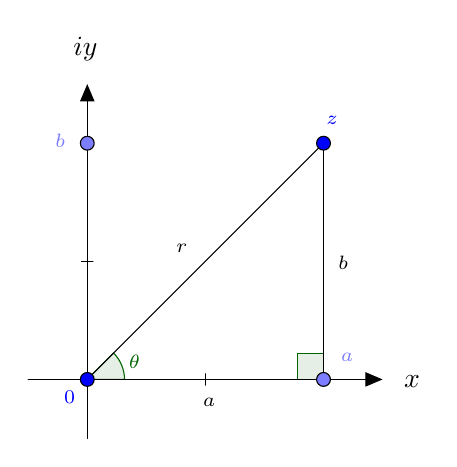
\begin{tikzpicture}[line cap=round,line join=round,>=triangle 45,x=1.5cm,y=1.5cm]
	\draw[->,color=black] (-0.5,0.) -- (2.5,0.);
	\foreach \x in {,1.,2.}
	\draw[shift={(\x,0)},color=black] (0pt,2pt) -- (0pt,-2pt);
	\draw[color=black] (2.6,-0.15) node [anchor=south west] {$x$};
	\draw[->,color=black] (0.,-0.5) -- (0.,2.5);
	\foreach \y in {,1.,2.}
	\draw[shift={(0,\y)},color=black] (2pt,0pt) -- (-2pt,0pt);
	\draw[color=black] (-0.2,2.8) node [anchor=west] {$iy$};
	\clip(-0.5,-0.5) rectangle (2.5,2.5);
	\draw[color=qqwuqq,fill=qqwuqq,fill opacity=0.1] (2.,0.22277768022923544) -- (1.7772223197707646,0.22277768022923547) -- (1.7772223197707646,0.) -- (2.,0.) -- cycle;
	\draw [shift={(0.,0.)},color=qqwuqq,fill=qqwuqq,fill opacity=0.1] (0,0) -- (0.:0.3150552167742013) arc (0.:45.:0.3150552167742013) -- cycle;
	\draw (0.,0.)-- (2.,2.);
	\draw (2.,2.)-- (2.,0.);
	\draw (0.,0.)-- (2.,0.);
	\begin{scriptsize}
	\draw [fill=qqqqff] (2.,2.) circle (2.5pt);
	\draw[color=qqqqff] (2.0719752655925316,2.191528364493368) node {$z$};
	\draw [fill=qqqqff] (0.,0.) circle (2.5pt);
	\draw[color=qqqqff] (-0.15,-0.15) node {$0$};
	\draw[color=black] (0.8012525579365867,1.109838786901943) node {$r$};
	\draw [fill=xdxdff] (2.,0.) circle (2.5pt);
	\draw[color=xdxdff] (2.2,0.185676817697619) node {$a$};
	\draw[color=black] (2.1664918306247922,0.9838167001922624) node {$b$};
	\draw [fill=xdxdff] (0.,2.) circle (2.5pt);
	\draw[color=xdxdff] (-0.22792781685913763,2.023498915547127) node {$b$};
	\draw[color=black] (1.0322930502376675,-0.19238944243142264) node {$a$};
	\draw[color=qqwuqq] (0.4,0.15) node {$\theta$};
	\end{scriptsize}
	\end{tikzpicture}
\end{figure}

When we plot it, we get a triangle with vertices $0,a,z$.
If we consider the line $az$, we see that it is parallel to the $iy$ axis, which is in turn perpendicular to the $x$ axis.
Thus, $\triangle 0az$ is right and $r=\sqrt{a^2+b^2}$ by Pythagorean theorem.
We also define $|z|=\sqrt{a^2+b^2}$, or the Euclidean distance between $z$ and $0$.

Furthermore, consider the angle $\theta$.
If we use the change of variables $a=r\cos\theta$ and $b=r\sin\theta$, we get that $\theta = \arctan(b/a)$.
Thus, we can write $z=a+bi$ as $r(\cos\theta+i\sin\theta)$, which gives us a polar representation of $z$.
Moreover, we call $r$ the \textit{modulus} of $z$ and $\theta$ the \textit{argument} of $z$; note that both the modulus and argument are real numbers.

\section{Euler's Formula}

In the 1740's Leonhard Euler noted that
\[
	e^{ix}=\cos x + i\sin x.
\]
We provide a proof of that.
\begin{thm}
	Let $x\in\RR$ and $i$ be the positive root of $x^2+1$.
	Then $e^{ix} = \cos x + i \sin x$.
\end{thm}
\begin{proof}
	We know $e^{ix}$ is a complex number thus, $e^{ix}=r\cdot(\cos \theta+ i\sin \theta)$, where $r=r(x)$ and $\theta = \theta(x)$.
	Therefore
	\[
		\frac{d}{dx} e^{ix} = \frac{d}{dx}\paren{r\cdot\paren{\cos \theta+ i\sin \theta}}
	\]
	and
	\[
		-r\sin\theta + ir\cos\theta =
		ie^{ix} =
		\paren{\cos \theta+ i\sin \theta}\frac{dr}{dx} + r\cdot\paren{-\sin \theta+ i\cos \theta}\frac{d\theta}{dx}.
	\]
	Thus, when we match real and imaginary parts, we get
	\[
		\cos \theta\frac{dr}{dx} - r\sin\theta\frac{d\theta}{dx} = -r\sin\theta
	\]
	and
	\[
		\sin \theta\frac{dr}{dx} + r\cos\theta\frac{d\theta}{dx} = r\cos\theta.
	\]
\end{proof}

\section{The Unit Circle}

\end{document}
